\documentclass[12pt, a4paper]{report}
\usepackage[margin=1in]{geometry}
\usepackage{graphicx}

\graphicspath{desktop}
\usepackage{imakeidx}
\makeindex

\title{\textbf{\underline{SMART TO-DO LIST}}}

\date{22 november 2019}

\begin{document}
\begin{titlepage}

\centering
{\scshape\bfseries\LARGE SOFTWARE REQUIREMENT SPECIFICATION (SRS) \par}
\vspace{1cm}
{\scshape\bfseries\huge SMART TO-DO LIST \par}
\vspace{1cm}
{\scshape\bfseries\huge Version 1.0 \par}
\vspace{2cm}
{\LARGE\bfseries Abdul Ahad (CS-17022) \par}
\vspace{1cm}
{\LARGE\bfseries Syedah Nawal Munif (CS-17024) \par}
\vspace{1cm}
{\LARGE\bfseries Sanjna Rajani (CS-17089) \par}
\vspace{2.5cm}
{\Large\itshape Department of Computer and Information Systems \\ NED University of Engineering and Technology\par}

\vfill
Submitted to\par
Ms. Fakhra Aftab \textsc
\vfill
% Bottom of the page
{\large Novemeber 21, 2019 \par}
	
\end{titlepage}


\tableofcontents

\chapter{INTRODUCTION}
Smart to do list  is an open source to-do manager specially designed to help users manage their tasks and  projects without going through the process of typing. It is available in English and works majorly on voice commands. The project has been developed in C\#. 
\section{DOCUMENT PURPOSE \index{Document Scope}}
A Software Requirements Specification (SRS) is a document that describes what the software will do and how it will be expected to perform. This Software Requirements Specification provides a complete description of all the functions and specifications of the smart to do list.  
Todo apps are widely used, but different users use the apps differently depending on their particular needs.
The main purpose of this smart to-do list is that it provides ease to users as it helps users to set their tasks or any important meeting to be reminded of by using their voice commands and the algorithm then processes the natural human language into computer understandable language and set the reminder of the particular task for the user. It reduces human efforts of typing and without going through the process of providing every detail to the system, the user can just say the sentence along with date and time and the system will automatically set it for user.
\newpage
\section{PROJECT SCOPE \index{Project Scope}}
\subsection{DESCRIPTION}
To do list is a practical organizing tool for all types of users. For common users or business oriented users , as it has the capability to work as a plain manager or as a professional to-do manager.
\subsection{BENEFITS}
As a plain to do manager,  user’s tasks can be saved and reminded in hierarchical form. While, as a professional to do manager, timers are set which can aid to remind of the meetings schedules and also of the approaching deadlines.
here are many benefits of To Do lists, from helping you prioritize your time to helping you remember what it is you meant to do! Manage tasks effectively. You can see all of the items at a glance and prioritize, what most needs to be done according to timelines and importance.
\section{INTENDED AUDIENCE \index{Intended Audience}} 
The SRS document is addressed to:  
\begin{itemize}
	\item Developers  who want to extend the program with new features. 
	\item Testers  who are interested in discovering possible flaws of the program and want to report them for improvement. 
	\item All users of the program, who are interested in being informed about the capabilities, which smart to-do list, gives to them.  
\end{itemize}
\section{DOCUMENT OVERVIEW \index{Overview}}
The rest of this SRS 
\begin{itemize}
	\item chapter 2 gives a general description of the project. It gives what level of capability is anticipated from the client, some broad requirements while making the product and a few suppositions and conditions that are accepted. 
	\item chapter 3 contains most significant highlights of the project portraying detail description and requirements. It explicitly states the requisites which the product is required to convey.  Functional requirements are given in this section. This area is composed essentially for the developers and portrays in specialized terms the functioning of the project, security performance and execution.
	\item chapter 4 consists of non-functional requirements describing them in detail.
	\item chapter 5 comprises of database information.
\end{itemize}
\section{DEFINITIONS, ACRONYMS AND ABBREVIATIONS}
\textbf{\underline{SQL Server}} \newline \newline SQL stands for Structured Query Language \index{SQL}. SQL is a database computer language designed for managing data in relational database management systems (RDBMS), and originally based upon relational algebra and calculus. Its scope includes data insert, query, update and delete, schema creation and modification \index{schema}, and data access control. \newline \textbf{\underline{.NET framework}} \newline \newline .NET Framework \index{.NET Framework} is a software framework developed by Microsoft that runs primarily on Microsoft Windows. It includes a large class library named as Framework Class Library and provides language interoperability across several programming languages.
\section{DOCUMENT CONVENTIONS}
In general this document follows the IEEE formatting requirements. font size 12 is used throughout the document for text. Document text issingle spaced .no special formatting techniques are used.
\section{REFERENCES AND ACKNOWLEDGEMENTS \index{refrences}}
\begin{itemize}
	\item https://krazytech.com/projects/sample-software-requirements-specificationsrs-report-airline-database
	\item http://todomoo.sourceforge.net/
	\item https://todoist.com/app
\end{itemize}

\newpage \chapter{OVERALL DESCRIPTION}
\section{PRODUCT PERSPECTIVE \index{Product Perspective}}
The product is supposed to be an open source. It is a desktop based system enhancing user to make their lives productive and manage time. This product is a follow-on and improved version dealing with certain ML algorithms which helps user to just create a reminder by voice recognition without the need of typing anything. It reduces the efforts of typing and will provide user delightful experience. Be it a meetup or some random office work, it will help in reminding every scenario with just human voice. \newline \newline 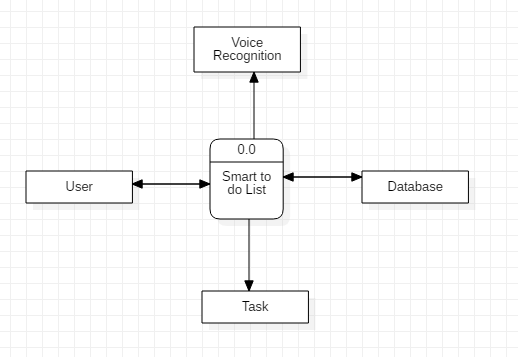
\includegraphics[scale=1.2]{dfd.png}
\newpage
\section{PRODUCT FUNCTIONALITY \index{Functionalities}}
The Intelligent ToDo System provides a simple mechanism for users to organize their daily routine by saying something like “Remind me to bring vegetables at 2pm” and it will smartly set the reminder and will prompt it to the user. \index{e.g}
\begin{itemize}
	\item Set a reminder to organize your day
	\item Set an alarm for meetings, milestones etc
	\item Reduce the effort of typing 
	\item Suggests time for the completion of task 
	\item Prioritize the most important task first
	\item Constantly reminding you to complete pending tasks (if any)
	\item Works with voice recognition
\end{itemize}

\section{USERS AND CHARACTERSTICS \index{End Users} \index{Intended Audience}}
This product will cover all the end-users whether a student or a company manager. Anyone can handle their tasks on the basis of their daily life functionalities. This will generally help people like manager or CEO, it basically works like a secretary as it will remind all the important meetings and milestones and focus on the most important conferences and piece of work first, prioritize on the basis of the company's benefit.
Students and people at home can find it useful to manage their daily life routine by setting an organized plan on the product with the ease of using their voice only to set the tasks. Anyone from the company's CEO to a teenage student, everyone can find this easy and handy who wants to make their lives organized and productive by keeping track at all times.
\section{OPERATION ENVIRONMENT \index{Operating System}}
This will work in any desktop environment, whether be it Windows, Linux , MacOS etc . There’s no explicitly system requirements as it is a very easy and not a hardcore software program. It is a local product so it doesn’t require any sort of server to store database. Everyone has their independence to work in the environment on their local PCs and the database is stored in the PC locally so only you can access it. As this product is developed on C\# and .NET Classes so it’s more of Windows compatible along with Linux and MacOS support.\newline  \newline \textbf{Minimum System Requirement} \index{System Requirements}
\begin{itemize}
	\item Processor: Intel Pentium 4 2.0GHz / AMD Athlon XP 2500+ 
	\item RAM: 512MB
	\item OS: Windows XP
	\item 3D: No
	\item Microphone: YES 
	\item Installed at least .NET Framework 3.50
\end{itemize}
\begin{center}
\section{DESIGN AND IMPLEMENTATION CONSTRAINTS \index{Constraints}}
\end{center}
This system is provisioned to be built on the .NET Classes which is highly flexible \index{.NET Framework}. Decision regarding which database to use should be taken considering the fact that data being stored is not large and stored locally. \newline The assumed factors that will affect the product is the use of microphone. In any case if the microphone is not in working condition, the whole idea of the project will go in vain as the main reason of using this intelligent ToDo is to just say your task and it will know what time to set and when to remind you. Another constraint that may arise is voice recognition API, we’re using voice recognition API \index{API} to fetch the human natural language and then after applying some algorithms translated into text and then applying machine learning to set the task to be reminded so if the API crashes due to some error or bug, the whole product will be of no use. Also the factor of noise in the environment is also a major issue if the software can not listen properly what the end user is trying to say, it may end up messing up things. The overloaded of tasks is another thing to keep in mind if the user keeps on adding task without finishing the old one so the system will prompt user to constraint for now and complete old tasks.


\section{USER DOCUMENTATION \index{Document Scope} \index{End Users} \index{Intended Audience}}
There’s not such user documentation needed for this product as this product is pretty simple and everyone of every age group can easily hold a grasp on it. Adding the task you wish to work on and provide the deadline is all you want to do for this product to work. The rest will be handled by the ToDo program. All you need to know is what task you should be reminded of and when and the ToDo assured everything for you.

\section{ASSUMPTIONS AND DEPENDENCIES \index{Constraints}}
It purely depends on the voice recognition API which is doing most of the work and is the base of this system. However, ML algorithms \index{ML algorithms} to set tasks efficiently is used later in the system to make this ToDo not any ordinary ToDo software product but an efficient and smarter one. You need to make assumptions in a project to be able to move forward with it. As we’ve established, planning is never certain and there are many external factors you can’t control or anticipate. The dependency on the .NET Framework classes \index{.NET Framework} is another thing to take into account which helps us to develop the product without the need of starting and defining each and every thing from scratch. The documentation by Microsoft is also being considered when working with C\# and .NET Classes to develop this system.
\newpage
\chapter{SPECIFIC REQUIREMENTS}
\section{EXTERNAL INTERFACE REQUIREMENTS}
\subsection{USER INTERFACES \index{User Interfaces}}
The first interface available to user will be of home page displaying a button that proceeds further. \newline For example \newline The user will then be directed to another screen in which he/she can add tasks through voice commands, schedule them or delete them. \newline Example:
\subsection{HARDWARE INTERFACES \index{Hardware Interfaces}}
The logical characteristics of each interface between the hardware and the user of the system is all handled by C\# and .NET Library as it helps the computer in computing the instructions provided by the developer and the compiler processed that instructions and provides information to the computer to perform the following tasks. It plays a big role in human-computer interaction as it reduces one of the main barriers of language between human and computer.	\newline All ToDo system needed is a Windows machine since C\# is developed by Microsoft so it provides a great means of ecosystem for the environment.
\subsection{SOFTWARE INTERFACES \index{Software Interfaces} \index{System Requirements}}
Not a lot has been going on in software interface, all it needs is a Windows machine and MS Visual Studio and all the work is being carried out by the developer. Since this product is mostly used by the users for personal or professional attitude of work, so it doesn’t need to have large or distributed database. To keep things simple, we’re going with local database because anyone using ToDo system is using it for its own productivity and simplicity and for example: if a company makes it obvious to use ToDo system, Even so everyone will be using it in their personal computer organizing their personal or professional life. \newline The preferred OS used for this product is Windows just because of the ecosystem although you can also run this on Linux or MacOS without any issue.
\subsection{COMMUNICATION INTERFACE \index{Cross Platform Support}}
The Smart TO-DO project  will be locally available. neither the cloud service is involved nor the cross platform support.
\section{FUNCTIONAL REQUIREMENTS \index{Functional Requirements}}
Functional requirements may involve calculations, technical details, data manipulation and processing, and other specific functionality that define what a system is supposed to accomplish.
\begin{enumerate}
	\item \textbf{\underline{TASK}} \newline In this menu there are many features regarding the task in the to do list. Features in this category are about creating, editing and managing tasks.  \newline  \begin{enumerate}\item \underline{NEW TASK} \newline \newline \textbf{USER REQUIREMENT}\newline  \newline User will add a task. User can set a new task either manually or through voice command. User can say set a task “meeting” on “2nd october 2019” at 3:00pm” or Task name, date and time can be set up manually. User can also add reminding option in which he/she will be reminded of the task completion prior to the deadline. \newline \newline \textbf{SYSTEM REQUIREMENTS} \index{System Requirements} \index{Add Tasks Support}
	\begin{enumerate}
	\item The user will select the add task option.
	\item Add task page will be opened consisting of minimum three fields.
	\item First field will be add task name.
	\item Second field will be date of task completion.
	\item Third field will be time of task completion.
	\item When the user presses add, system must check if the “name”, “date” and “time”  fields  are completed.
	\item The fields can be typed-in or can be entered through voice command.
	\item The task will be stored in database.
	\item  If they are not, it should warn the user that the particular field is mandatory, and allow the user to continue completing.
	\end{enumerate}

	\item \underline{EDIT TASK} \index{Edit Task Support} \newline \newline \textbf{USER REQUIREMENTS} \newline \newline The user must select any task for the previously existing tasks and can edit its name, date or day. \newline \newline \textbf{SYSTEM REQUIREMENTS} \index{System Requirements}
	\begin{enumerate}
	\item The user will select the edit task option.
	\item Edit task page will opened.
	\item User may change name, date or day of the existing task.
	\item Edited task cannot be saved if the new name of it is empty.
	\item If there is not a task selected before user chooses edit task option, the task cannot be saved.
	\item The edited information will be updated in the database.
	\end{enumerate} 

	\item \underline{DELETE TASK} \index{Delete Tasks Support} \newline \newline \textbf{USER REQUIREMENTS} \newline \newline In this feature, it is described how the user can delete a task.    \newline \newline \textbf{SYSTEM REQUIREMENTS} 
	\begin{enumerate}
	\item User selects a task Then chooses “Task: Delete task” . 
	\item the system will then ask/confirm if the user wants to delete the selected task. 
	\item If user answers positive, then this task  will be deleted, else the delete command will be canceled
	\end{enumerate}
	\end{enumerate}

	\item \textbf{\underline{VIEW}} \newline In this menu there are features, which select the view of the tasks. \newline  \begin{enumerate} \item \underline{COMPLETED TASKS} \newline \newline \textbf{USER REQUIREMENT}\newline  \newline in this feature, it is described, how users can show the completed tasks.  User chooses “View: Show completed tasks”. \newline \newline \textbf{SYSTEM REQUIREMENTS} 
	\begin{enumerate}
	\item User chooses the option to view tasks.
	\item User will select the option of view completed tasks.
	\item System must show any task that is completed in the task list.
	\item User must not be able to choose show completed tasks, if these tasks are already shown. 
	\end{enumerate}

	\item \underline{INCOMPLETED TASKS} \newline \newline \textbf{USER REQUIREMENT}\newline  \newline In this feature, users can view uncompleted task.  \newline \newline \textbf{SYSTEM REQUIREMENTS} 
	\begin{enumerate}
	\item User chooses the option to view tasks.
	\item User will select the option of view incompleted tasks.
	\item When the user chooses to utilize this feature, system must show any task which is pending.
	\item If all the tasks are already completed, no taskk will appear in this view option.
	\end{enumerate}
	\end{enumerate}

	\item \textbf{\underline{SMARTLY DIVIDED IN CATEGORIES}} \newline \begin{itemize} \item \textbf{FUNCTION} \newline The smart To Do system can smartly defines the category of task and combines all the task of the same category in one place.

	 \item \textbf{DESCRIPTION} \newline \index{End Users} This would help the students or businessmen to manage their household and school/office tasks easily. Also, the completed and pending tasks are pre-defined in different categories so you can always take a quick glance on the completed or pending tasks. 

	\item \textbf{INPUTS} \newline the user will give input by selecting any of the available categories. 

	\item \textbf{SOURCE OF INPUT} \newline user will give input in this feature by selecting the category. 

	\item \textbf{OUTPUTS}\newline The output of this feature will be in the form that tasks will be displayed or can be viewed in different categories. 

	\item \textbf{ACTION} \newline as the user selects a particular category for a particular tast, databse will be updated i.e the particular category will be assigned to that task. 

	\item \textbf{PRE-CONDITION} \newline There is no pre-condition to utilize this feature. 

	\item \textbf{POST-CONDITION} \newline after selecting a particular category, user must enter task name, date and time to store it in database. 

	\item \textbf{EXCEPTION} \newline if the task name, date or day is not assigned, then the task will not be updated under the selected category inn database and hence cannot be viewed. 
\end{itemize}


	\item \textbf{\underline{ALARM TONE}} \newline \newline \textbf{USER REQUIREMENTS} \newline \newline In this feature, user can select any of the alarm tone provided by the system. \index{Alarm Support}  \newline \newline \textbf{SYSTEM REQUIREMENTS} 
	\begin{enumerate}
	\item User can choose any of the available alarm tone.
	\item The system should remind the user of the task by ringing the specific tone selected by the user.
	\end{enumerate}

\section{BEHAVIOUR REQUIREMENTS}
\subsection{USE CASE VIEW \index{Use Case View}}

Here there’s only one actor but we can further specify it like Student, Manager and Teacher. For the sake of simplicity, we’re considering User who can add tasks with respective date and time using their voice commands and also edit , view and delete the tasks. Moreover, tasks are then classified into categories depending on the type of tasks. \newline \newline 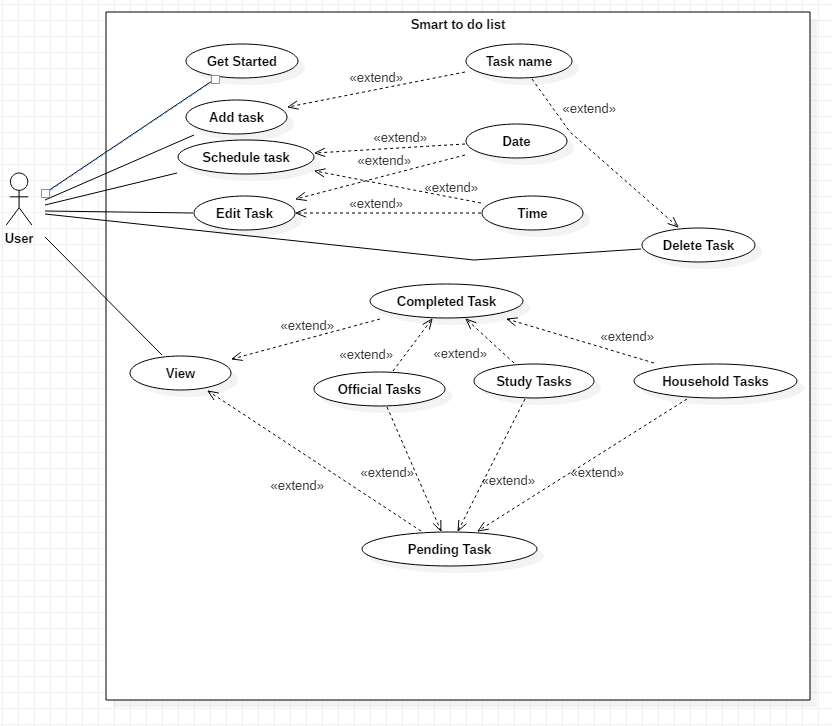
\includegraphics[scale=0.61]{usecase.png}


\chapter{OTHER NON-FUNCTIONAL REQUIREMENTS}
\section{PERFORMANCE REQUIREMENTS \index{System Requirements}}
Smart to do list is a program with :
\begin{itemize}
	\item Minimal memory requirements, 
	\item Disk space and
	\item Processing power. 
	\item However to use the voice command feature, the microphone should be working.
	\item Any task can be edited provided that it is not completed.
	\item Any task whether completed or not, can be deleted.
\end{itemize}
\section{SAFETY AND SECURITY REQUIREMENTS \index{Safety} \index{Security}}
The program should be of the greatest possible use to the public, the best way to achieve this is to make it free software which everyone can redistribute.
\begin{itemize}
	\item To do so,it is safest to each files at least the “copyright” line.
	\item Also add information on how to contact you by electronic and paper mail.
	\item Database should be protected by a username and password.
\end{itemize}
However, .NET framework classes are open to all and can be used by any user. \index{.NET Framework}
\section{SOFTWARE QUALITY ATTRIBUTES \index{SQA}}
\subsection{EFFICIENCY}
The program aims to provide the user ease and functionality without any charge. It lets you keep track of everything in one place, so you can get it all done and enjoy more peace of mind along the way.
\subsection{USABILITY}
Our software is user friendly. It can be used for the professional employees as well as by the unemployed people and students. It can be used in diverse ways.
\subsection{ECOSYSTEM}
This software provides a great means of ecosystem. By developing this product on native platforms, you can work on cross platforms. You can update, delete and edit tasks from your Windows PC or mobile phones and even from car multimedia control system but our main focus is towards windows platform so we only implement that. We can further make it work on cross platforms across different OS.
\subsection{OPERATIONAL}
The smart to-do list also offers an essential non functional requirement highlighting the operation of the software. The software will only be operational when a user is registered. No guest accounts are allowed.

\chapter{DATABASE REQUIREMENTS \index{SQL} \index{Database} \index{Database Requirements}}
Keeping in mind the database is saved locally, it’s not a large or distributed database. Tables and entities are divided in terms of categories like Pending tasks and Completed Tasks and further subdivided into Household chores, Official Work etc. 
The preferred database system we’re using is sql since it’s minimal and handy to use for such a small database. Moreover, no specific or hardcore server is required for this purpose as it’s consuming very little memory and can easily fit in any PC.

\end{enumerate}
\newpage


\printindex

\end{document}